\documentclass[12pt]{article}
\usepackage{hyperref}
\usepackage{amsmath, amssymb, amsfonts}
\usepackage[margin=1.2cm]{geometry}
\usepackage{xcolor}
\usepackage{graphicx}
\usepackage{enumitem}
\parindent 0pt
\newcommand{\lb}{\\$\left|\rightarrow\right.$}
\newcommand{\enter}{\\\textcolor{white}{1}}
\ExplSyntaxOn
\NewDocumentCommand{\bo}{m}
 {
   \bold_commas:n { #1 }
 }
\cs_new:Npn \bold_commas:n #1
 {
   \seq_set_split:Nnn \l_tmpa_seq { , } { #1 }
   \seq_map_indexed_function:NN \l_tmpa_seq \__bold_commas_aux:nn
 }
\cs_new:Npn \__bold_commas_aux:nn #1 #2
 {
   \textbf{#2}
   \int_compare:nNnTF { #1 } < { \seq_count:N \l_tmpa_seq }
     { , }
     { }
 }
\ExplSyntaxOff

\title{Digital Signal Analysis and Processing (CT704)\\[0.2em]
\large and Digital Signal Processing (EX753)\\[0.4em]
\large Detailed PYQ \quad 2066--2082}
\author{}
\date{\today}

\begin{document}
\maketitle
\vspace{4cm}
\textbf{Notes}
\begin{itemize}[noitemsep]
  \item Two papers are combined in this one document:
    \begin{itemize}[noitemsep]
      \item \textbf{CT704} --- \emph{Digital Signal Analysis and Processing}, BEI/BCT, Year/Part IV/I. 27 papers, \bo{2066 Magh} to \bo{2082 Bhadra}. Shown in the \textbf{normal} font. (The three oldest papers carry no subject code; 2069 Bhadra is coded EG774CT.)
      \item \textbf{EX753} --- \emph{Digital Signal Processing}, BEX, Year/Part IV/II. 17 papers, \bo{2069 Bhadra} to \bo{2081 Chaitra}. Shown in \texttt{typewriter}. (2069 Bhadra is coded EG773EX.)
    \end{itemize}
  \item Programme is the \texttt{typewriter} axis, exam type is the bold axis --- the two are independent:\\
    \bo{76 Ch} = CT704 Regular \qquad 76 Ash = CT704 Back\\
    \bo{\texttt{76 Bh}} = EX753 Regular \qquad \texttt{74 Ma} = EX753 Back
  \item Regular exam = \bo{bold}, Back exam = regular font. ``New Back (2066 \& Later Batch)'' counts as Back. A header printing ``Regular / Back'' in one cell is treated as Regular.
  \item Months: Ba = Baishakh, Jth = Jestha, Asa = Ashad/Ashar, Shr = Shrawan, Bh = Bhadra, Ash = Ashwin, Ka = Kartik, Mng = Mangsir, Po = Poush, Ma = Magh, Ch = Chaitra.\\
    Note \bo{70 Asa} (2070 Ashad, CT704) and 75 Ash (2075 Ashwin, CT704) are different months --- do not merge them.
  \item Keywords: (I) = Importance/Need, (+) = Advantage, (-) = Disadvantage, +Fig = Figure, +Eg = Example, Vs = Compare/Differentiate.
  \item Marks kept in [brackets] as originally split (e.g.\ [2+6]).
  \item Chapters 1--7 are the CT704 syllabus chapters, in syllabus order, with the official hour count printed under each. Chapter 8 collects the topics that lie outside that syllabus and are set only by \texttt{EX753} (DSP fundamentals, A/D quantization, DSP processors). Sampling questions belong to Chapter 1 (syllabus 1.10) and are filed there.
  \item Every question statement here is reproduced \textbf{in full}, with all its given data. Nothing is abbreviated. Where the original paper itself omits data or misprints a symbol, that is stated in place.
\end{itemize}
\pagebreak
\tableofcontents
\pagebreak

%=======================================================================
\section{Discrete-Time Signals and Systems}
\begin{center}(8 Hours)\end{center}

  \subsection{Basic signals, even/odd, transformation of variable}
    \begin{enumerate}[topsep=0pt, noitemsep]
      \item Define even and odd type discrete time signals with suitable example. Plot the signal $x[-2n+3]$ where $x[n]=\{1,2,0,-1,-3,-4\}$. \hfill [2+3] (\bo{76 Ch})

      \item Find the even and odd part of the signal $x[n]=\{1$ for $-4\le n\le0;\ 2$ for $1\le n\le4\}$. \hfill [3] (\bo{71 Ch}, 70 Asa)
        \lb Find the odd and even part of the signal shown in the stem plot below \hfill [4+5] (71 Shr)\\
        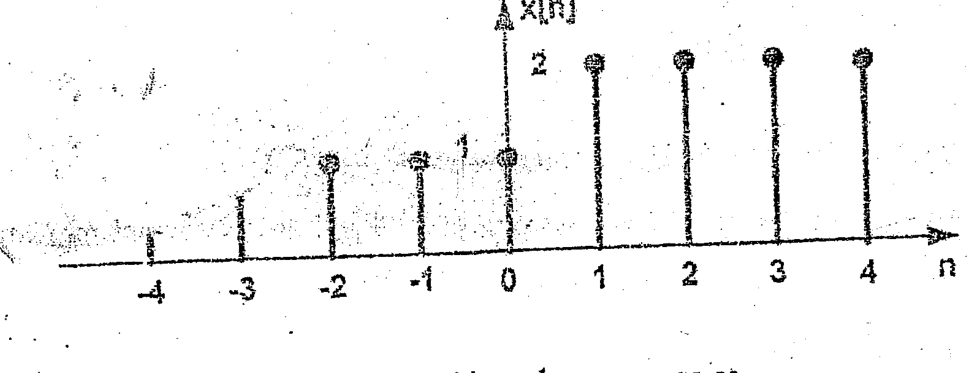
\includegraphics[width=4in]{images/dsap_71shr_stem.png}\\
        and, for the same question: a discrete time LTI system has input signal and impulse response $x[n]=\{1$ for $-1\le n\le1$; 0 elsewhere$\}$ and $h[n]=\{1$ for $-1\le n\le1$; 0 elsewhere$\}$. Find the output of the system using the graphical method.
        \lb Compute and plot even and odd component of the sequence $x(n)=2u[n]-2u[n-4]$, where $u[n]$ is unit step sequence. \hfill [2] (\bo{67 Mng})

      \item Define and plot a discrete time unit step signal. Explain its relation with the unit impulse signal. \hfill [1+2] (\bo{73 Ch})

      \item Plot the sequence $x[n]=u[n]-u[n-3]+5\delta[n-4]+nu[n-6]$. List out the properties of LTI system. \hfill [3+2] (\bo{74 Ch})
        \lb Plot the sequence $x(n)=u(n)-u(n-5)+5\delta(n-6)+nu(n-7)-nu(n-9)$, where $u(n)$ is the unit step sequence and $\delta(n)$ is unit sample sequence. \hfill [2] (\bo{66 Ma})
        \lb Plot the sequence $x[n]=u[n+8]-u[n-4]$. \hfill [3] (\bo{69 Bh})
    \end{enumerate}

  \subsection{Energy / power signals and periodicity}
    \begin{enumerate}[topsep=0pt, noitemsep]
      \item Define (compare) energy and power signal, and determine whether the given signal is periodic (find its fundamental period).
        \lb $x[n]=\cos(2\pi n/5)+\sin(\pi n/3)$ \hfill [2+2] (\bo{79 Bh, 69 Ch, 81 Bh}) --- in \bo{81 Bh} the definition part is dropped and only the periodicity is asked \hfill [4]
        \lb $x[n]=e^{j(\pi n/3+\pi/4)}$ \hfill [2+2] (74 Ash)
        \lb $x[n]=e^{j(\pi n/2+4\pi/7)}$: is it an energy signal or a power signal? \hfill [2+2] (79 Ba, \bo{82 Bh})
        \lb $x[n]=u[n]$ and $x[n]=\delta[n]$: energy or power type? \hfill [2+3] (72 Ka)
        \lb Find the energy and power of the signal $x[n]=u[n]$. \hfill [5] (\bo{68 Bh})
        \lb Power Vs energy signal; Fourier Series Vs Fourier Transform. \hfill [3+4] (\bo{75 Ch})
        \lb Differentiate between energy and power, period and aperiodic, symmetric and anti-symmetric signals. Check whether the following signal is linear or non-linear: $y[n]=x^2[n]$. \hfill [3+3] (\texttt{74 Ma})

      \item Determine whether the signal is periodic; if periodic, state its periodic/fundamental time.
        \lb $x[n]=e^{j\pi n/16}\cos(n\pi/17)$ \hfill [5] (\bo{80 Bh})
        \lb (a) $\sin(n\pi)+\cos(n\pi)$ \quad (b) $\sin(3n\pi/5)+\cos(4n\pi/7)$ \hfill [2+2] (80 Ba)
        \lb $x[n]=\cos(\pi n/2)\cos(\pi n/4)$ \hfill [4] (\bo{78 Bh})
        \lb (i) $\cos(\pi n^2/8)$ \quad (ii) $\cos(n/2)\cos(\pi n/4)$ \hfill [3] (\bo{70 Ch})
        \lb What is the period of the following signals? (a) $x[n]=\cos(11\pi n/3)$ \quad (b) $x[n]=e^{j(7/5)n}$ \hfill [4] (\bo{69 Bh})
        \lb Write whether or not the following sequences are periodic and write the period. (a) $x[n]=\cos(5\pi n/3)$ \quad (b) $x[n]=\sin(\pi n/\sqrt{2}+\pi/8)$ \hfill [4] (\bo{67 Mng})
        \lb Write whether or not the following sequences are periodic and write the period. (a) $x(n)=\cos(\tfrac{3\pi}{8}n+\tfrac{\pi}{4})$ \quad (b) $x(n)=\sin(0.8n)$ --- printed in the paper as ``sing(0.8n)''. \hfill [4] (\bo{66 Ma})
    \end{enumerate}

  \subsection{System properties (linearity, time-invariance, causality, stability)}
    \begin{enumerate}[topsep=0pt, noitemsep]
      \item A DT system is given by $y(n)=\sum_{k=0}^{n}x(k)$; check whether it is memoryless, time-invariant and stable. \hfill [2+2+2] (\bo{80 Bh})

      \item Determine the given systems: (a) $y[n]=x[-n]$: time-invariant? (b) $y[n]=x[n^2]$: linear? \hfill [5] (\bo{76 Ch})
        \lb (a) $y[n]=y[n-4]+x[n-4]$: time-invariant? (b) $y[n]=x^2[n]$: linear? \hfill [3+3] (\bo{74 Ch})
        \lb $y[n]=y[n-4]+x[n-4]$: time invariant or not? \hfill [3] (\bo{\texttt{78 Ch}})
        \lb (a) $y[n]=x^2[n]$ (b) $y[n]=\cos(\tfrac{5\pi}{8}n+\tfrac{\pi}{4})$: linear or not? \hfill [3+3] (75 Ash)
        \lb Determine whether the following systems are (a) causal (b) linear: (i) $y[n]=x[n]-3x[n-1]$ \quad (ii) $y[n]=x[n+1]+4x[n]$ \hfill [4] (\bo{\texttt{71 Bh}})
        \lb Determine whether the following systems are (a) causal (b) linear and (c) time invariant: (i) $y(n)=\log_{10}[\{x(n)\}]$ \quad (ii) $y(n)=x(-n-2)$ \hfill [5] (\bo{\texttt{70 Bh}})

      \item An LTI system is given by $y(n)=x(n)+e^{a}y(n-1)$; check this system for BIBO stability. \hfill [5] (81 Ba)

      \item State whether or not the system $y[n]=e^{x[2n]}$ is (a) linear (b) time invariant (c) memoryless (d) causal, where $x[n]$ is input to system and $y[n]$ is output of system. \hfill [5] (\bo{68 Bh})
        \lb Show whether or not the system $y(n)=nx[2(n-2)]$, $n>0$ is (a) linear, (b) time invariant, (c) memoryless. \hfill (marks clipped in the scan) (\bo{67 Mng})
        \lb Show whether or not the following systems are (a) linear; (b) time invariant, (c) causal, (d) memoryless, (e) BIBO stable: (a) $y(n)=2^{\log_2(x(n))}+2^{\log_2(x(n))}$ \quad (b) $y(n)=\sin\{x(n)-x(n-1)\}$ \hfill [10] (\bo{66 Ma})
        \lb Write about the following properties of discrete time system: [a] linearity, [b] time invariance, [c] memory, [d] causality, [e] stability. \hfill [5] (\bo{69 Bh})

      \item Explain the properties of LTI systems with suitable examples. \hfill [8] (\bo{\texttt{72 Ash}})
        \lb Explain the conditions for an LTI/LSI system to be causal and BIBO (Bounded Input Bounded Output) Stable. \hfill [6] (\texttt{70 Ma})
        \lb Define recursive and non-recursive system with suitable examples. State the condition for the stability and causality of LTI system in terms of ROC and pole zero. \hfill [3+3] (\bo{\texttt{74 Bh}})
        \lb Draw the recursive form of a moving average system. \hfill [5] (\texttt{70 Ma})
    \end{enumerate}

  \subsection{Fourier series / transform of DT signals}
    \begin{enumerate}[topsep=0pt, noitemsep]
      \item Explain the process of calculating Fourier series coefficients. \hfill [3] (73 Shr); How are Fourier series coefficients calculated? Explain. \hfill [4] (\bo{72 Ch})

      \item Explain the Fourier transform multiplication property for two sequences. Write Dirichlet's conditions for Fourier series. \hfill [4+3] (76 Ash)

      \item Find the expression for discrete Fourier series of the sequence $x(n)=\sum_{m=-\infty}^{\infty}\delta(n-4m)$. \hfill [4] (\bo{66 Ma})
        \lb Find the period of the signal $x[n]=\sum_{m=-\infty}^{\infty}\delta[n-2-3m]$. Find the Fourier series coefficients of the signal $x[n]$. \hfill [6] (\bo{68 Bh})
        \lb Find the discrete Fourier coefficients of the periodic sequence with period $N=11$ defined over a period as $x[n]=\{1,\ |n|\le2;\ 0,\ 2<|n|\le5\}$. \hfill [4] (\bo{67 Mng})
    \end{enumerate}

  \subsection{Convolution --- output of an LTI system}
    \begin{enumerate}[topsep=0pt, noitemsep]
      \item What is a convolution summation? Derive its equation and explain it. \hfill [1+3] (\bo{\texttt{69 Bh}}); What is a convolution sum and derive its equation? \hfill [3] (\texttt{73 Ma})
        \lb Illustrate the significance of convolution summation in digital signal analysis. \hfill [2] (70 Asa, \bo{\texttt{70 Bh}})

      \item Find the output $y(n)$ of an LTI system given its impulse response $h$ and input $x$ (convolution). Each parameter set below is a separate paper.
        \lb $h(n)=\{5,4,3,2\},\quad x(n)=\{1,0,3,2\}$ \hfill [6] (\bo{70 Ch})
        \lb $h(n)=\{1,1,1\},\quad x(n)=\{1,1,1,1\}$ \hfill [6] (73 Shr)
        \lb $h(n)=\{1,1,1\},\quad x(n)=\{1,-2,2,3,4\}$ \hfill [2+4] (\bo{\texttt{70 Bh}})
        \lb $h(n)=\{1,0,1\},\quad x(n)=\{1,-2,-2,3,4\}$ \hfill [2+4] (70 Asa)
        \lb $h(n)=\{2,2,-1,1\},\quad x(n)=\{1,2,1,2\}$ \hfill [6] (\bo{\texttt{74 Bh}})
        \lb $h[n]=\{5,3,4,2,0\},\quad x[n]=\{0,2,4,6\}$ (FIR system response) \hfill [5] (\texttt{74 Ma})
        \lb $h(n)=\{1,3,2,-1,1\}$ for $-1\le n\le3,\quad x(n)=2\delta(n)-\delta(n-1)$ \hfill [6] (\bo{71 Ch})
        \lb $x[n]=\delta[n]+2\delta[n-1]-\delta[n-3],\quad h[n]=2\delta[n+1]+2\delta[n-1]$ \hfill [5] (\bo{79 Bh, 81 Bh})
        \lb $h[n]=(1/2)^n\{u[n+2]-u[n-2]\},\quad x[n]=\{2,1,0,-1,4\}$ \hfill [5] (79 Ba)
        \lb $h[n]=(1/2)^n\{u[n+2]-u[n-2]\},\quad x[n]=\{2,1,0.5,-1\}$; also check the answer \hfill [3+2] (74 Ash)
        \lb $h[n]=0.5^n\{u[n]-u[n-3]\},\quad x[n]=\{2,1,0.5,-1\}$ \hfill [5] (\bo{82 Bh})
        \lb $h[n]=(1/3)^n\{u[n+1]-u[n-2]\},\quad x[n]=\{2,1,0.5,3\}$ \hfill [5] (72 Ka)
        \lb $h[n]=2^n\{u[n]-u[n-3]\},\quad x[n]=\delta[n]+\delta[n-1]+\delta[n-2]$ \hfill [5] (75 Ash)
        \lb $h[n]=2^n\{u[n]-u[n-3]\},\quad x[n]=\delta[n]+\delta[n-1]-\delta[n-3]$ \hfill [4+6] (\bo{\texttt{79 Ch}, \texttt{75 Bh}})
        \lb $h[n]=u[n]-u[n-4],\quad x[n]=(1/2)^n u[n]$ \hfill [5] (\bo{78 Bh})
        \lb $h[n]=u[n+1]-u[n-4],\quad x[n]=(1/2)^n u[n]$ \hfill [2+6] (\texttt{73 Ma})
        \lb $h[n]=u[n+1]-u[n-3],\quad x[n]=(0.5)^n u[n]$ \hfill [6] (\bo{\texttt{78 Ch}})
        \lb $h[n]=(1/2)^n u[n-1],\quad x[n]=u[n+1]-u[n-4]$ \hfill [6] (\bo{76 Ch})
        \lb $h[n]=2u[n]-2u[n-4],\quad x[n]=(1/3)^n u[n]$ \hfill [1+4] (\bo{69 Ch})
        \lb $h[n]=2u[n]-2u[n-5],\quad x[n]=(1/3)^n u[n]$ \hfill [2+2+6] (\bo{\texttt{81 Ch}, \texttt{80 Ch}}); [8] (\texttt{72 Ma})
        \lb $h[n]=2u[n+2]-2u[n-3],\quad x[n]=(1/3)^n u[n-1]$ \hfill [2+6] (\bo{\texttt{76 Bh}})
        \lb $h[n]=2u[n+3]-2u[n-4],\quad x[n]=(1/2)^n u[n+1]$ \hfill [3+7] (\bo{\texttt{77 Ch}})
        \lb $h(n)=(1/3)^n u(n-3),\quad x(n)=(1/6)^{n-6}u(n)$ \hfill [6] (81 Ba)
        \lb $h[n]=(1/3)^n u[n],\quad x[n]=5e^{j\pi n/2}$ for $-\infty<n<\infty$ \hfill [4] (\bo{70 Ch})
        \lb $h[n]=(1/2)^n u[n],\quad x[n]=5e^{j\pi n/3}$ for $-\infty<n<\infty$ \hfill [4] (72 Ka); [5] (80 Ba)
        \lb $h[n]=(1/2)^n u[n],\quad x[n]=Ae^{jn\pi}$ \hfill [2+3+5] (71 Shr)
        \lb $h[n]=(1/2)^n u[n],\quad x[n]=Ae^{jn\pi/2}$ \hfill [2+4] (\bo{\texttt{69 Bh}})
        \lb $h[n]=(1/2)^n u[n],\quad x[n]=10-5\sin(\pi n/2)+20\cos(\pi n)$, $-\infty<n<\infty$ \hfill [3+7] (73 Shr)
        \lb $x[n]=a^n u[-n]$ with $0<a<1,\quad h[n]=u[n]$ \hfill [6] (76 Ash) --- the paper prints this as ``$2^n4[-n]$'' and ``$4[n]$''
        \lb $x[n]=3^n u[-n-5],\quad y[n]=u[n-5]$ \hfill [5] (\bo{68 Bh})
        \lb $x[n]=\{1$ for $0\le n\le4$; 0 otherwise$\},\quad h[n]=\{a^n$ for $0\le n\le6$; 0 otherwise$\}$, $a>1$ \hfill [8] (\bo{\texttt{73 Bh}})

      \item Find the output of an LTI system whose impulse response and input are given as tabulated values; also check/verify the result.
        \lb $x[-2]=0.5,\ x[0]=1,\ x[1]=0.75,\ x[3]=0.5$; $h[0]=1,\ h[1]=0.75,\ h[2]=0.5$ (the paper writes $h$ as ``$n[n]$'') \hfill [6] (\bo{73 Ch})
        \lb $h[-2]=3,\ h[0]=2,\ h[1]=1$; $x[n]=2^n$ for $-1\le n\le3$ \hfill [5+2] (\bo{75 Ch})
        \lb $h[-2]=1,\ h[0]=2,\ h[1]=3$; $x[0]=1/2,\ x[2]=2,\ x[3]=3$ \hfill [3+2] (\bo{72 Ch})
        \lb Given as stem plots: $h[0]=0.5,\ h[1]=0.75,\ h[2]=1$; $x[-2]=1,\ x[0]=0.5,\ x[2]=1,\ x[3]=0.75$ (zero at $n=-1$ and $n=1$) \hfill [7] (\bo{\texttt{71 Bh}})\\
        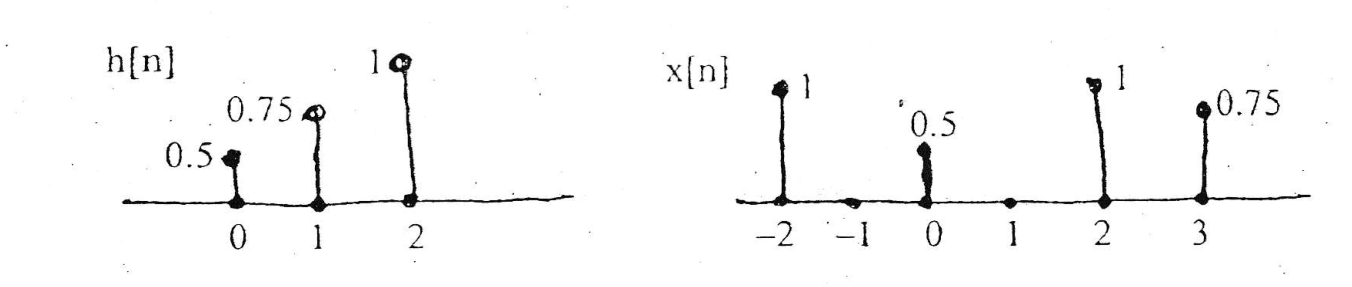
\includegraphics[width=5in]{images/dsap_71bh_ex753_stem.png}
    \end{enumerate}

  \subsection{Sampling of continuous-time signals, spectral properties of sampled signal}
    \begin{enumerate}[topsep=0pt, noitemsep]
      \item What is a sampling? How are the spectrum of continuous time signal and the spectrum of signal obtained by sampling the continuous time signal related? Illustrate with diagram. \hfill [6] (\bo{69 Bh})
        \lb How is the spectrum of continuous time signal related to spectrum of corresponding discrete time signal obtained by sampling the continuous time signal? Explain. Discuss what is aliasing and how it occurs. \hfill [8] (\bo{68 Bh})

      \item Consider the analog signal $x_a(t)=3\cos 100\pi t$.
        \begin{enumerate}[label=(\alph*), noitemsep, topsep=0pt]
          \item Determine the minimum sampling rate required to avoid aliasing.
          \item Suppose that signal is sampled at $F_s=75$ Hz. What is the discrete time signal obtained after sampling?
          \item Assume now that we sample this signal using a sampling rate $F_s=5{,}000$ samples/sec. What is discrete time signal after sampling?
        \end{enumerate}
        \hfill [1+3+3] (\bo{\texttt{81 Ch}}); [7] (\texttt{74 Ma})
        \lb Same signal $x(t)=3\cos(100\pi t)$, only two parts: (a) minimum sampling rate to avoid aliasing; (b) if sampled at $F_s=200$ Hz, what is the discrete time signal obtained after sampling? Also list out the advantages of digital signal processing over analog signal processing. \hfill [2+2+3] (\bo{\texttt{78 Ch}})

      \item Define causal and stable system with examples. Consider a continuous time signal $x(t)=\sin 2000\pi t-5\cos 12000\pi t+10\sin 6000\pi t$. What is the discrete time signal obtained after sampling the signal at a sampling rate of 5000 samples per second for $0\le n\le 3$? \hfill [3+4] (\bo{\texttt{80 Ch}})
        \lb Explain the general application areas of digital Signal Processing. Consider a continuous time signal $x(t)=\sin 2000\pi t+5\cos 12000\pi t+10\sin 6000\pi t$. What is the discrete time signal obtained after sampling the signal at a sampling rate of 5000 samples per second for $0\le n\le 3$? \hfill [3+4] (\bo{\texttt{73 Bh}})
        \lb Consider a continuous time signal $x(t)=\cos 1000\pi t+3\sin 3000\pi t+5\cos 5000\pi t$. Calculate the discrete time signal for sampling rate of 6000 samples per second for $0\le n\le 3$. \hfill [4] (\texttt{73 Ma})

      \item List out the major disadvantages of Digital Signal Processing. When does oversampling occur? Consider the analog signal $x(t)=3\cos 50\pi t+10\sin 300\pi t-0.7\cos 100\pi t$:
        \begin{enumerate}[label=(\alph*), noitemsep, topsep=0pt]
          \item What is the Nyquist rate for this signal?
          \item Suppose that the signal is sampled at the rate of $F_s=5000$ samples per second, what is the discrete-time signal obtained after sampling?
          \item What is the analog signal we can reconstruct from the samples?
        \end{enumerate}
        \hfill [2+1+1+2+2] (\bo{\texttt{76 Bh}})

      \item Why do you need anti-aliasing filter? Describe the effect of sample and hold circuit at the input of the A/D conversion of Discrete Time Processing of continuous time signal. \hfill [2+5] (\bo{\texttt{69 Bh}})
    \end{enumerate}

\pagebreak
%=======================================================================
\section{Z-Transform}
\begin{center}(4 Hours)\end{center}

  \subsection{ROC --- definition and properties}
    \begin{enumerate}[topsep=0pt, noitemsep]
      \item Define ROC / state and explain the properties of Region of Convergence. \hfill [1--5] (\bo{80 Bh, 73 Ch, 72 Ch, 81 Bh, \texttt{77 Ch}, \texttt{71 Bh}, \texttt{70 Bh}}, 79 Ba, 72 Ka, 71 Shr)
        \lb Define ROC. Explain the properties of ROC with suitable examples. \hfill [1+4] (\bo{\texttt{73 Bh}})
        \lb State the properties of region of convergence (ROC). Obtain the z-transform of the following signal: $x[n]=na^n u[n]$. \hfill [2+4] (\bo{\texttt{78 Ch}})
        \lb Define one sided Z-transform. Find Z-transform of $x[n]=na^n u[n]$ using properties. Also mention ROC of this signal. \hfill [5] (\texttt{70 Ma})
        \lb Write the properties for Region of Convergence (ROC). A discrete-time signal is expressed as $x[n]=\cos\omega n$ for $n\ge0$. Find its Z-transform. \hfill [3+8] (\texttt{74 Ma})

      \item Properties of ROC, and locate the ROC of the given signal:
        \lb $x[n]=(-1/3)^n u[n]-(1/3)^n u[-n-1]$ \hfill [2+4] (\bo{70 Ch}, 70 Asa)
        \lb $x[n]=(0.6)^n u[n]+(0.25)^n u[n]$ \hfill [3+6] (75 Ash)
        \lb $x[n]=(0.1)^n u[n]+(0.3)^n u[-n-1]$ \hfill [4+6] (\bo{75 Ch})
        \lb $x[n]=(0.25)^n u[n]+(0.6)^n u[-n-1]$ \hfill [4+6] (\bo{\texttt{75 Bh}})
        \lb $x[n]=(0.5+j0.2)^n u[n]+(-j)^n u[-n-1]$: find $X(z)$ at $z=0.4$ and $z=0.7$, where $X(z)$ is the bilateral Z-transform of $x[n]$. \hfill [1+4] (\texttt{73 Ma})
    \end{enumerate}

  \subsection{Properties of Z-transform (convolution, time-shift, scaling)}
    \begin{enumerate}[topsep=0pt, noitemsep]
      \item State the convolution property of Z-transform (and derive/prove it). \hfill [3+3/3+6/2+4] (76 Ash, 72 Ka, 70 Asa, \texttt{72 Ma})
        \lb State and prove convolution property of z-transform. Describe causality and stability of system in terms of ROC with suitable examples. \hfill [1+3+3] (\bo{\texttt{72 Ash}})
      \item Derive the time shifting property of Z-transform. \hfill [3+3] (\bo{69 Ch})
      \item Define Z-transform. How is it related to DTFT? Explain scaling property of Z-transform with suitable example. \hfill [3+3] (\bo{\texttt{74 Bh}})
      \item List out the properties of z-transform. \hfill [2] (\bo{\texttt{76 Bh}})
      \item Explain one sided Z-transform with its importance. Explain the time delay property of one sided Z-transform. \hfill [3+3] (\texttt{73 Ma})
    \end{enumerate}

  \subsection{Inverse Z-transform (partial fraction / long division)}
    \begin{enumerate}[topsep=0pt, noitemsep]
      \item Determine the inverse Z-transform for the given $X(z)$ and ROC. Each line is one paper's parameter set.
        \lb $H(z)=\dfrac{1+2z^{-1}+z^{-2}}{1-0.75z^{-1}+0.125z^{-2}}$, ROC $0.25<|z|<0.5$ \hfill [1+6] (\bo{80 Bh})
        \lb $X(z)=\dfrac{1}{1-0.8z^{-1}+0.12z^{-2}}$ for (i) $|z|>0.6$, (ii) $|z|<0.2$, (iii) $0.2<|z|<0.6$ \hfill [2+2+3] (81 Ba)
        \lb $X(z)=\dfrac{1+2z^{-1}+z^{-2}}{1-1.5z^{-1}+0.5z^{-2}}$, ROC $|z|>1$ \hfill [1+5] (80 Ba)
        \lb $X(z)=\dfrac{1+2z^{-1}+z^{-2}}{1+1.5z^{-1}+0.5z^{-2}}$, $|z|>1$, by partial fractions \hfill [6] (71 Shr)
        \lb $X(z)=\dfrac{1+2z^{-1}+z^{-2}}{1+4z^{-1}+4z^{-2}}$: determine the causal signal $x[n]$ \hfill [6] (\bo{\texttt{80 Ch}, \texttt{70 Bh}}); by long division for all possible ROCs \hfill [6] (\texttt{70 Ma})
        \lb $X(z)=\dfrac{2z^4+2z^3-3z+2}{z^2-1.5z-1}$, ROC $|z|<0.5$, by partial fraction expansion \hfill [6] (\bo{79 Bh})
        \lb $X(z)=\dfrac{2z^3-5z^2+z+3}{(z-1)(z-2)}$, ROC $|z|<1$, by partial fraction expansion \hfill [1+5] (\bo{81 Bh})
        \lb $H(z)=\dfrac{z}{3z^2-4z+1}$, $\tfrac13<|z|<1$, by partial fraction \hfill [1+5] (79 Ba, \bo{82 Bh})
        \lb $X(z)=\dfrac{z^3+z^2+1.5z+0.5}{z^3+1.5z^2+0.5z}$, ROC $|z|<1/2$ \hfill [1+5] (\bo{78 Bh})
        \lb $X(z)=\dfrac{z^4+5z^3-3z+4}{z^2-1.5z-1}$, ROC $|z|<0.5$ \hfill [2+6] (\bo{76 Ch})
        \lb $X(z)=\dfrac{z^4+z^3-3z+5}{z^2-1.5z-1}$, ROC $|z|<0.5$ \hfill [6] (\bo{\texttt{81 Ch}, \texttt{71 Bh}})
        \lb $X(z)=\dfrac{z^4-2z^3-z+4}{z^2-1.5z-1}$, ROC $|z|<0.5$ \hfill [6] (\bo{\texttt{79 Ch}})
        \lb $X(z)=\dfrac{z^4+2z^3-z+4}{z^2-1.5z-1}$, ROC $|z|<0.5$ \hfill [5] (\bo{\texttt{72 Ash}})
        \lb $X(z)=\dfrac{z}{(z-0.6)(z+0.5)^2}$, ROC $|z|>0.6$ \hfill [3+6] (76 Ash)
        \lb $X(z)=\dfrac{z}{(z-0.4)(z+1.5)^2}$, ROC $|z|<0.4$ \hfill [1+5] (73 Shr)
        \lb $X(z)=\dfrac{z}{(z-1)(z-2)^2}$, ROC $|z|<1$ \hfill [1+5] (70 Asa)
        \lb $X(z)=z^2\big[1-\tfrac32 z^{-1}\big](1+z^{-1})(1-z^{-1})$ \hfill [3+3] (74 Ash)
        \lb $X(z)=z^2(1-1.5z^{-1})(1-z^{-1})(1+z^{-2})$ \hfill [4] (\bo{\texttt{78 Ch}})
        \lb $X(z)=\dfrac{2z^3+2z^2+3z+5}{z^2-0.1z-0.2}$, ROC $|z|<0.4$ \hfill [1+3+5] (\bo{74 Ch, 73 Ch, \texttt{74 Bh}}) --- all three papers misprint the leading term as $2z^2$
        \lb $X(z)=\dfrac{1}{(z-0.5)(z+2)}$ for (i) $0.5<|z|<2$, (ii) $|z|<0.5$, (iii) $|z|>2$ \hfill [1+5] (\bo{71 Ch})
        \lb $X(z)=\dfrac{1}{1-0.5z^{-1}+1.5z^{-2}}$, ROC $|z|>1$, by long division \hfill [6] (\bo{\texttt{77 Ch}})
        \lb $X(z)=\dfrac{1}{1-1.58z^{-1}+0.5z^{-2}}$ by long division, when ROC $|z|>1$ and when ROC $|z|<\tfrac12$ \hfill [2+6] (\bo{\texttt{76 Bh}})
        \lb $X(z)=\dfrac{1}{1-\tfrac32 z^{-1}+\tfrac12 z^{-2}}$ by long division, when ROC $|z|>1$ and when ROC $|z|<\tfrac12$ \hfill [6] (\bo{\texttt{73 Bh}})
        \lb $X(z)=\dfrac{1}{1-1.5z^{-1}+0.5z^{-2}}$ for (a) ROC $|z|>1.5$ and (b) ROC $|z|<0.5$ \hfill [6] (\texttt{72 Ma})
        \lb $H(z)=\dfrac{1-\tfrac12 z^{-2}}{(1-\tfrac12 z^{-1})(1-\tfrac14 z^{-1})}$, $|z|>1/2$: determine the impulse response of the system \hfill [6] (\bo{\texttt{69 Bh}})
    \end{enumerate}

\pagebreak
%=======================================================================
\section{Analysis of LTI Systems in Frequency Domain}
\begin{center}(6 Hours)\end{center}

  \subsection{Pole--zero plot and magnitude / phase response}
    \begin{enumerate}[topsep=0pt, noitemsep]
      \item Plot the pole-zero in the z-plane and draw the magnitude response (not to scale) of the system described by the given difference equation:
        \lb $y(n)=x(n)+0.8x(n-1)+0.8x(n-2)+0.49y(n-2)$ \hfill [3+7] (\bo{80 Bh})
        \lb $y(n)=0.67x(n)-0.3x(n-1)+2.75y(n-1)$ \hfill [3+7] (81 Ba); phase response instead of magnitude \hfill [2+8] (76 Ash)
        \lb $y[n]-0.35y[n-1]+0.25y[n-2]=x[n]-0.75x[n-1]$ \hfill [3+7] (\bo{79 Bh})
        \lb $y[n]-0.3y[n-1]+0.2y[n-2]=x[n]-0.5x[n-1]$ \hfill [3+7] (79 Ba)
        \lb $y[n]-0.4y[n-1]+0.25y[n-2]=x[n]-0.4x[n-1]$ \hfill [2+4] (\bo{78 Bh}); \hfill [3+7] (\bo{81 Bh})
        \lb $y[n]-0.4y[n-1]+0.25y[n-2]=x[n]+0.5x[n-1]$ (magnitude response only) \hfill [8/7] (\bo{\texttt{80 Ch}, \texttt{72 Ash}})
        \lb $y[n]-0.4y[n-1]+0.2y[n-2]=x[n]+0.5x[n-1]+0.6x[n-2]+0.8x[n-3]$ \hfill [3+7] (74 Ash)
        \lb $y[n]-0.5y[n-1]+0.3y[n-2]=x[n]+0.7x[n-1]$ \hfill [6] (72 Ka)
        \lb $y[n]-0.4y[n-1]+0.1y[n-2]=x[n]+0.6x[n-1]$ \hfill [2+4] (\bo{72 Ch})
        \lb $y[n]-0.3y[n-1]+0.225y[n-2]=x[n]+0.5x[n-1]$ \hfill [6] (\bo{70 Ch})
        \lb $y[n]-0.3y[n-1]+0.225y[n-2]=x[n]-0.4x[n-1]$ \hfill [6] (\bo{\texttt{71 Bh}})
        \lb $y[n]-0.3y[n-1]+0.2y[n-2]=x[n]+0.7x[n-1]$ \hfill [7] (\texttt{73 Ma})
        \lb $y[n]-0.4y[n-1]+0.2y[n-2]=x[n]+0.1x[n-1]-0.06x[n-2]$ \hfill [2+2+6] (\bo{69 Ch})
        \lb $y[n]-0.6y[n-1]+0.35y[n-2]=x[n]-0.1x[n-1]-0.2x[n-2]$ \hfill [2+5] (\bo{\texttt{76 Bh}})
        \lb $y(n)-0.3y(n-1)=2x(n-2)+0.7x(n-1)+4x(n)$ \hfill [2+7] (\bo{75 Ch})
        \lb $y[n]-0.8y[n-1]+0.15y[n-2]-x[n]=0$: find the frequency response $H(e^{j\omega})$ and plot it. \hfill [6] (\bo{69 Bh})
        \lb $y[n]-\tfrac56 y[n-1]-\tfrac16 y[n-2]-x[n]=0$: find $H(z)$, its poles and zeros, and use the pole-zero diagram to plot the approximate frequency response magnitude. \hfill [10] (\bo{67 Mng})
        \lb $y[n]-\tfrac{10}{24}y[n-1]+\tfrac{1}{24}y[n-2]=x[n]$: find the frequency response, then determine $y[n]$ for the input $x[n]=\sin(\tfrac{\pi}{3}n)+\sin(\tfrac{\pi}{5}n)$. \hfill [7] (\bo{68 Bh})
        \lb $y[n]=x[n]+1.21x[n-2]-0.8y[n-1]$: explain how the poles and zeros of $H(z)$ affect stability and gain response, plot poles/zeros on the z-plane, determine whether the system is causal and stable, and sketch its gain response. \hfill [3+3+2+4] (\bo{\texttt{69 Bh}})
        \lb $y(n)=x(n)+x(n-2)$: plot poles and zeros, determine the magnitude response, and determine whether the system is causal and stable. \hfill [2+6+2] (70 Asa); magnitude \emph{and phase} response \hfill [8] (\texttt{70 Ma})

      \item Map the poles and zeros in the z-plane and plot the magnitude response for a system with the given pole/zero locations:
        \lb poles $0.45\pm j1.6$, zeros $0.58\pm j2.06$ \hfill [4+6] (80 Ba); \hfill [2+8] (\bo{82 Bh})
        \lb poles $0.45\pm j1.06$, zeros $0.58\pm j2.06$ \hfill [2+6] (\bo{76 Ch}); [2+8] (75 Ash); [8] (\bo{\texttt{81 Ch}, \texttt{73 Bh}})
        \lb poles $0.45-0.77i$ and $-2\pm0.3i$ \hfill [2+8] (\bo{74 Ch})
        \lb poles $0.45-0.77i$ and $-2\pm0.3i$, zeros $1.2\pm3i$ \hfill [2+6] (\bo{\texttt{75 Bh}})
        \lb poles $0.45+0.77i$ and $2\pm0.7i$, zeros $1.2\pm0.43i$ \hfill [2+8] (\bo{73 Ch})
        \lb poles $0.45+0.77i$ and $-2\pm0.3i$, zeros $1.2\pm3i$ \hfill [2+8] (\bo{71 Ch})
    \end{enumerate}

  \subsection{FIR vs IIR, LCCDE, linear phase, stability / causality}
    \begin{enumerate}[topsep=0pt, noitemsep]
      \item Differentiate between FIR system and IIR system. \hfill [4] (80 Ba, \bo{\texttt{76 Bh}})
        \lb How does an IIR filter differ from an FIR filter? \hfill (marks clipped in the scan) (\bo{67 Mng})
      \item State linear constant coefficient difference equation and the corresponding system function. \hfill [3] (73 Shr, 71 Shr)
        \lb Why do we need difference equation? \hfill [2] (71 Shr, \bo{69 Ch, \texttt{69 Bh}})
        \lb Define the difference equation with example. \hfill [2] (\bo{73 Ch})
      \item Determine the zero-input response for the second order system $y[n]-3y[n-1]-4y[n-2]=x[n]$. \hfill [4] (\bo{78 Bh})
        \lb Let a system be characterized by the difference equation $y(n)-0.5y(n-1)-0.25y(n-2)-x(n)=0$, where the input is $x(n)=0.2^n u(n)$ and the initial conditions are $y(-1)=2$, $y(-2)=4$. Find (a) zero input response of the system, (b) zero state response of the system, (c) total response of the system, (d) system function $H(z)$, (e) poles of $H(z)$. \hfill [10] (\bo{66 Ma})
      \item Describe stability and causality characteristics of an LTI system in terms of Impulse Response and ROC of its transfer function with suitable examples. \hfill [4+3] (76 Ash); [4] (\bo{72 Ch})
        \lb Define a Causal and Stable system in terms of impulse response. \hfill [2] (\bo{\texttt{81 Ch}, \texttt{80 Ch}}, \texttt{73 Ma})
        \lb Define causal and stable system with examples. \hfill [3] (\bo{\texttt{73 Bh}})
        \lb Define causality and stability of LTI system in terms of impulse response with a suitable example. \hfill [3] (\bo{\texttt{77 Ch}})
      \item What is the condition satisfied by a linear phase FIR filter? Show that the filter with $h(n)=\{-1,0,1\}$ is a linear phase filter. \hfill [2+4] (70 Asa)
        \lb Show that the filter with impulse response $h[n]$, $0\le n\le N-1$, where $h[n]=h[N-1-n]$, is a linear phase filter. \hfill [6] (\bo{67 Mng})
        \lb Derive the expression for the frequency response of a symmetric linear phase filter of length $M$, where $M$ is odd. \hfill [6] (\bo{69 Bh})
    \end{enumerate}

\pagebreak
%=======================================================================
\section{Discrete Filter Structures}
\begin{center}(8 Hours)\end{center}

  \subsection{Direct form, cascade and parallel realizations}
    \begin{enumerate}[topsep=0pt, noitemsep]
      \item Obtain the Direct Form I and Direct Form II realization of the given system:
        \lb $y[n]-0.25y[n-2]=x[n]+0.4x[n-1]+0.5x[n-2]$ \hfill [2+2] (\bo{79 Bh})
        \lb $y[n]-0.75y[n-1]-0.25y[n-2]=x[n]+0.5x[n-1]$ \hfill [4] (79 Ba); \hfill [2+2] (\bo{82 Bh})
        \lb $3y[n]+y[n-1]+2y[n-4]=2x[n]+x[n-3]$ \hfill [5] (\bo{74 Ch})
        \lb $y(n)=-0.1y(n-1)+0.2y(n-2)+3x(n)+3.6x(n-2)+0.6x(n-2)$ \hfill [5] (\bo{72 Ch})
        \lb Direct Form II only: $y(n)=-0.1y(n-1)+0.72y(n-2)+0.7x(n)-0.252x(n-2)$ \hfill [4] (72 Ka, \bo{69 Ch})
        \lb $H(z)=\dfrac{(1-\tfrac15 e^{-j\pi/5}z^{-1})(1-\tfrac13 z^{-1})(1-\tfrac15 e^{j\pi/5}z^{-1})}{(1-\tfrac45 z^{-1})(1-\tfrac17 e^{j\pi/7}z^{-1})(1-\tfrac15 z^{-1})(1-\tfrac17 e^{-j\pi/7}z^{-1})}$ in terms of Direct Form I and Direct Form II structures; draw the corresponding block diagrams. \hfill [9] (\bo{68 Bh})

      \item Realize the given system in cascade form of second-order sections (signal flow graph):
        \lb Cascade of 2nd-order sections \hfill [5] (81 Ba)\\
          \mbox{}\hfill {\small $H(z)=\dfrac{10(1-0.25z^{-1})(1-0.667z^{-1})(1+2z^{-1})}{(1-0.75z^{-1})(1-0.125z^{-1})\{1-(0.5+j0.5)z^{-1}\}\{1-(0.5-j0.5)z^{-1}\}}$}\hfill\mbox{}
        \lb Cascaded \emph{and parallel} form \hfill [7] (\texttt{74 Ma})\\
          \mbox{}\hfill {\small $H(z)=\dfrac{5(1-0.25z^{-1})(1-0.667z^{-1})(1+2z^{-1})}{(1-0.75z^{-1})(1-0.125z^{-1})[1-(0.5+j0.5)z^{-1}][1-(0.5-j0.5)z^{-1}]}$}\hfill\mbox{}
        \lb Cascade of 2nd-order sections \hfill [4] (80 Ba)\\
          \mbox{}\hfill {\small $H(z)=\dfrac{(1-0.4z^{-1})(1+0.2z^{-1})(1-0.3e^{j\pi/6}z^{-1})(1-0.3e^{-j\pi/6}z^{-1})}{(1-0.5e^{j\pi/3}z^{-1})(1-0.5e^{-j\pi/3}z^{-1})(1+0.7e^{j\pi/4}z^{-1})(1+0.7e^{-j\pi/4}z^{-1})}$}\hfill\mbox{}
        \lb Cascade of 2nd-order sections \hfill [4] (\bo{76 Ch})\\
          \mbox{}\hfill {\small $H(z)=\dfrac{(1-0.5z^{-1})(1+0.35z^{-1})(1-0.3e^{j2n\pi/5}z^{-1})(1-0.3e^{-j2n\pi/5}z^{-1})}{(1-0.6e^{jn\pi/3}z^{-1})(1-0.6e^{-jn\pi/3}z^{-1})(1+0.5e^{j2n\pi/7}z^{-1})(1+0.5e^{-j2n\pi/7}z^{-1})}$}\hfill\mbox{}
        \lb $H(z)=\dfrac{2(1-0.4z^{-1})(1-0.5z^{-1})}{(1+0.2z^{-1})(1-0.25z^{-1})[1-(-0.5+j0.15)z^{-1}][1-(-0.5-j0.15)z^{-1}]}$ \hfill [7] (\bo{\texttt{77 Ch}})
        \lb $H(z)=\dfrac{1}{(1-0.5z^{-1})(1-0.7e^{-j\pi/4}z^{-1})(1-0.7e^{j\pi/4}z^{-1})(1-0.3z^{-1})}$; draw the block diagram of the cascade realization. \hfill [6] (\bo{69 Bh})
        \lb Realize the following in cascade form and draw the block diagram of the cascade realization. (The paper prints the last denominator factor with a $-j\pi/4$ exponent twice; the conjugate is meant.) \hfill (marks clipped in the scan) (\bo{67 Mng})\\
          \mbox{}\hfill $H(z)=\dfrac{(1-\tfrac13 z^{-1})(1-\tfrac14 z^{-1})(1-\tfrac18 z^{-1})}{(1-\tfrac56 z^{-1})(1-\tfrac16 z^{-1})(1-\tfrac34 e^{-j\pi/4}z^{-1})(1-\tfrac34 e^{+j\pi/4}z^{-1})}$\hfill\mbox{}
        \lb $y[n]-\tfrac34 y[n-1]+\tfrac18 y[n-2]-x[n]-2x[n-1]=0$ \hfill [4] (\bo{70 Ch})

      \item A system has an impulse response $h[n]=(0.5)^n u[n]+n(0.2)^n u[n]$. Determine the parallel form realization. \hfill [6] (\bo{\texttt{78 Ch}})
    \end{enumerate}

  \subsection{Lattice and lattice-ladder structures}
    \begin{enumerate}[topsep=0pt, noitemsep]
      \item Compute the lattice (or lattice-ladder) coefficients and draw the structure for the given system function; check stability where the paper asks.
        \lb $H(z)=1/(1-0.2z^{-1}+0.4z^{-2}+0.6z^{-3})$ \hfill [10] (\bo{80 Bh})
        \lb $H(z)=1/(1-0.525z^{-1}+0.6125z^{-2}+0.3z^{-3})$, check stability \hfill [4+2+1] (\bo{\texttt{81 Ch}, \texttt{72 Ash}})
        \lb $H(z)=1/(1-0.9z^{-1}+0.64z^{-2}-0.576z^{-3})$, check stability \hfill [4+2+1] (\bo{\texttt{79 Ch}}); compute and draw \hfill [8] (\bo{\texttt{69 Bh}})
        \lb $H(z)=1/(1-0.3z^{-1}+0.5z^{-2}+0.25z^{-3})$ \hfill [6+2] (\bo{\texttt{71 Bh}})
        \lb $H(z)=1/(1+2z^{-1}-3z^{-2}+4z^{-3})$ \hfill [6] (\texttt{70 Ma})
        \lb $H(z)=1/(1-0.01z^{-1}-0.23z^{-2}+0.5z^{-3})$, check stability \hfill [4+2+1] (\bo{71 Ch})
        \lb FIR $H(z)=1+(13/24)z^{-1}+(5/8)z^{-2}+(1/3)z^{-3}$, check stability \hfill [5] (81 Ba); Direct Form + Lattice \hfill [3+7] (\bo{78 Bh})
        \lb lattice-ladder $H(z)=(2-0.7z^{-1}+0.5z^{-2})/(1-0.3z^{-1}+0.25z^{-2})$ \hfill [6] (80 Ba, \bo{82 Bh})
        \lb lattice-ladder $H(z)=(1-0.4z^{-1}+0.25z^{-2})/(1-0.3z^{-1}+0.5z^{-2})$, check stability \hfill [6+1] (79 Ba)
        \lb lattice-ladder $H(z)=\dfrac{1+z^{-1}+z^{-2}}{(1+0.5z^{-1})(1+0.3z^{-1})(1+0.4z^{-1})}$ \hfill [6+4] (\bo{81 Bh})
        \lb lattice-ladder $H(z)=(0.5-2z^{-1}+3z^{-2})/(1-0.5z^{-1}-0.7z^{-2}+0.3z^{-3})$ \hfill [6+4] (\bo{76 Ch})
        \lb lattice-ladder $H(z)=(0.7-1.5z^{-1}+0.5z^{-2})/(1-0.5z^{-1}-0.7z^{-2}+0.3z^{-3})$ \hfill [6+3] (76 Ash)
        \lb lattice-ladder $H(z)=(0.62+0.42z^{-1}-0.25z^{-2})/(1+0.27z^{-1}+0.06z^{-2}-0.75z^{-3})$, check stability \hfill [5+1] (\bo{\texttt{74 Bh}})
        \lb lattice-ladder $H(z)=(0.6-0.45z^{-1}-0.25z^{-2})/(1+0.27z^{-1}+0.06z^{-2}-0.75z^{-3})$, check stability \hfill [7+1] (\bo{\texttt{75 Bh}})
        \lb lattice-ladder $H(z)=(0.5-0.4z^{-1}-0.2z^{-2})/(1+0.2z^{-1}+0.7z^{-2}-0.75z^{-3})$, comment on stability \hfill [7+2] (\bo{\texttt{77 Ch}})
        \lb lattice-ladder $H(z)=(0.5+0.65z^{-1}+0.2z^{-2})/(1-0.45z^{-1}+0.3z^{-2}+0.5z^{-3})$, check stability \hfill [6+1] (\texttt{73 Ma})
        \lb lattice-ladder $H(z)=(1-z^{-1}+0.5z^{-2})/(1+0.2z^{-1}-0.15z^{-2})$, comment on stability \hfill [6+2] (\bo{\texttt{78 Ch}})
        \lb lattice-ladder $H(z)=(0.5+2z^{-1}+0.6z^{-2})/(1-0.3z^{-1}+0.4z^{-2})$ (pole-zero system) \hfill [6] (70 Asa)
        \lb lattice-ladder $H(z)=\dfrac{\tfrac12+\tfrac13 z^{-1}+\tfrac14 z^{-2}+\tfrac15 z^{-3}}{1+\tfrac15 z^{-1}+\tfrac25 z^{-2}+\tfrac35 z^{-3}}$ \hfill [6] (\bo{66 Ma})
        \lb $H(z)=1/(3+(39/24)z^{-1}+(15/8)z^{-2}+(3/9)z^{-3})$; also represent $5/8$ and $-5/8$ in sign-magnitude, 1's complement and 2's complement format. \hfill [7+3] (75 Ash)
        \lb $H(z)=1/(1+\tfrac23 z^{-1}+\tfrac58 z^{-2}+\tfrac23 z^{-3}+z^{-4})$ (printed ``$H(t)$'') \hfill [9] (\bo{75 Ch})
        \lb $H(z)=\dfrac{1+\tfrac13 z^{-1}+\tfrac98 z^{-2}+\tfrac43 z^{-3}+z^{-4}}{1+\tfrac23 z^{-1}+\tfrac58 z^{-2}+\tfrac23 z^{-3}+z^{-4}}$ \hfill [10] (\bo{73 Ch})
        \lb FIR $H(z)=1+2z^{-1}+z^{-2}$ \hfill [5] (\bo{72 Ch})
        \lb FIR $H(z)=1+2z^{-1}+2z^{-2}+z^{-3}$ (convert into a lattice-ladder structure) \hfill [6] (\bo{\texttt{73 Bh}})
        \lb FIR $H(z)=A_3(z)=1+(52/96)z^{-1}+(25/40)z^{-2}+(1/3)z^{-3}$ \hfill [5] (\bo{74 Ch})
        \lb Direct Form + Lattice, FIR $H(z)=1+0.7z^{-1}+1.2z^{-2}-z^{-3}$ \hfill [3+7] (74 Ash)
        \lb Direct Form + Lattice, $H(z)=2+1.8z^{-1}-1.6z^{-2}+z^{-3}$ \hfill [3+7] (73 Shr)
        \lb Direct Form + Lattice, $H(z)=1+2z^{-1}+0.62z^{-2}+0.8z^{-3}$ \hfill [2+5] (\bo{\texttt{76 Bh}})
        \lb FIR $H(z)=1+2z^{-1}-3z^{-2}+4z^{-3}$ \hfill [6] (72 Ka, \bo{69 Ch})
        \lb FIR $H(z)=1+3.1z^{-1}+5.5z^{-2}+4.2z^{-3}+2.3z^{-4}$ \hfill [6] (\bo{70 Ch})
        \lb $H(z)=2.3+\tfrac{3.6}{24}z^{-1}+\tfrac{101}{8}z^{-2}+\tfrac23 z^{-3}$ (the paper prints the third term with a positive exponent) \hfill [8] (\texttt{72 Ma})
        \lb All-pass filter $H(z)=\dfrac{1+0.4z^{-1}-1.2z^{-2}+2z^{-3}}{2-1.2z^{-1}+0.4z^{-2}+z^{-3}}$: show how to use a lattice structure to implement it. \hfill [8] (\bo{\texttt{70 Bh}})

      \item Given a 3-stage lattice filter with coefficients $K_1=1/4$, $K_2=1/2$, $K_3=1/3$ (all-zero / all-pole polynomial), obtain the system function and the FIR filter coefficients. \hfill [6] (\bo{79 Bh}); [5] (71 Shr)
        \lb Same, but with $K_1=1/4$, $K_2=1/4$, $K_3=1/3$: determine the FIR filter coefficients for the direct-form structure. \hfill [7] (\bo{\texttt{80 Ch}}, \texttt{74 Ma})
    \end{enumerate}

  \subsection{Quantization effects, number representation, limit cycles}
    \begin{enumerate}[topsep=0pt, noitemsep]
      \item What is the limit cycle effect in a recursive system? Describe with an example showing how it occurs. \hfill [3] (\bo{71 Ch}); [1+3] (70 Asa)
        \lb Define limit cycle oscillation. Explain it taking an example of an ideal single pole recursive system. \hfill [5] (\texttt{72 Ma})
        \lb What are the Round-off effects in Digital Filters? Explain Limit Cycle Oscillation with an example. \hfill [3+4/2+4] (\bo{\texttt{81 Ch}, \texttt{80 Ch}, \texttt{70 Bh}})
        \lb For the first order filter $y(n)=Q\{a\,y(n-1)\}+x(n)$, the product term ``$a\,y(n-1)$'' has been quantized by rounding it to 3 bits, with $y(-1)=0$, $x(n)=0.875\delta(n)$, $a=-0.5$. Show whether the filter goes into limit cycle. What is the period of the limit cycle? \hfill [4] (\bo{66 Ma})
      \item What is the importance of quantization in DSP? Which one is better, rounding or truncation? Explain about limit cycles in a recursive system. Define dead band. \hfill [1+1+2+1] (71 Shr)
      \item Write about the sign magnitude and 2's complement representation of a binary fractional number. Write about truncation error and rounding error. \hfill [6] (\bo{69 Bh})
        \lb Define one's complement, 2's complement and sign magnitude representation of numbers. Represent $-192/220$ in 8 bit 1's complement and 2's complement form. \hfill [3+4] (\bo{\texttt{69 Bh}})
        \lb Show by giving examples that the quantization error by truncation for a sign magnitude number, $e_{tsm}$, lies in the range $-(2^{-b}-2^{-b_u})\le e_{tsm}\le(2^{-b}-2^{-b_u})$ and that for the 2's complement number, $e_{t2c}$, lies in the range $-(2^{-b}-2^{-b_u})\le e_{t2c}\le0$, where $b_u$ is the number of bits before quantization and $b$ is the number of bits after quantization. \hfill (marks clipped in the scan) (\bo{67 Mng})
    \end{enumerate}

\pagebreak
%=======================================================================
\section{FIR Filter Design}
\begin{center}(6 Hours)\end{center}

  \subsection{Window method and Gibbs phenomenon}
    \begin{enumerate}[topsep=0pt, noitemsep]
      \item Describe how a digital FIR filter is designed by the window method (discuss the characteristics of the different window functions). \hfill [4+4] (\bo{70 Ch}); [5+3] (\bo{72 Ch}); [4] (\texttt{72 Ma}); [5] (\bo{\texttt{70 Bh}})

      \item Design a symmetric / linear-phase FIR low pass filter whose desired frequency response is $H_d(\omega)=e^{-j\omega\tau}$ for $|\omega|\le\omega_c$ and $0$ elsewhere. The length of the filter should be 7 and $\omega_c=1$ rad/sample.
        \lb using the Hanning window \hfill [10] (\bo{80 Bh}); with ``list out the key points of windowing'' \hfill [2+7] (\bo{\texttt{73 Bh}})
        \lb using the Blackman window, with ``What is windowing? List out the key points of windowing'' \hfill [1+2+7] (\bo{\texttt{76 Bh}})

      \item Design a low pass FIR filter using a suitable window for the given edge frequencies and stop band attenuation:
        \lb $\omega_p=0.2\pi$, $\omega_s=0.45\pi$, $\alpha_s=51$ dB \hfill [5+3] (79 Ba)
        \lb $\omega_p=0.3\pi$, $\omega_s=0.5\pi$, $\alpha_s=40$ dB \hfill [8] (\bo{71 Ch, 69 Ch})
        \lb $\omega_p=0.2\pi$, $\omega_s=0.5\pi$, $\alpha_s=41$ dB --- find the first six coefficients of the impulse response; also, why is Kaiser better than other fixed windows? \hfill [2+6] (74 Ash)
        \lb $\omega_p=0.24\pi$, $\omega_s=0.54\pi$, $\alpha_s=42.2$ dB --- find the first three coefficients of the impulse response \hfill [8] (\bo{\texttt{79 Ch}}); [6] (\bo{\texttt{75 Bh}})
        \lb $\omega_p=0.35\pi$, $\omega_s=0.45\pi$, stop-band attenuation of at least 54 dB \hfill [8] (\bo{67 Mng})
        \lb Hanning window, $\omega_p=0.25\pi$, $\omega_s=0.35\pi$, main-lobe width $8\pi/M$ where $M$ is the filter length \hfill [9] (70 Asa)
        \lb Hanning window, $\omega_p=0.25\pi$, $\omega_s=0.3\pi$ \hfill [8] (\bo{69 Bh})
        \lb Blackman window, $\omega_p=0.24\pi$, $\omega_s=0.34\pi$, main-lobe width of the Blackman window $12\pi/M$ where $M$ is the filter length \hfill [9] (\bo{68 Bh})

      \item Design an FIR filter using a suitable window for the following specifications:
        $0.899\le|H(e^{jw})|\le1$ for $|w|\le0.2\pi$; \quad $|H(e^{jw})|\le0.01$ for $0.4\pi\le|w|\le\pi$.
        \hfill [6] (\bo{76 Ch}); with ``Define Gibbs phenomena'' \hfill [2+6] (\bo{\texttt{81 Ch}}); with the Remez exchange algorithm \hfill [4+5] (\texttt{73 Ma})

      \item Explain Gibbs phenomenon / oscillation --- how it arises when the rectangular window is used in FIR filter design, and how it can be minimized. \hfill [3+3/5/6/1+4/2+5] (81 Ba, 80 Ba, 73 Shr, 71 Shr, \bo{\texttt{79 Ch}, \texttt{74 Bh}, \texttt{71 Bh}})
    \end{enumerate}

  \subsection{Kaiser window design}
    \begin{enumerate}[topsep=0pt, noitemsep]
      \item Why is the Kaiser window better than other fixed windows in FIR filter design? / Explain the steps to design an FIR filter using the Kaiser window. \hfill [3/4/7] (81 Ba, 74 Ash, \bo{72 Ch}, \bo{\texttt{80 Ch}, \texttt{72 Ash}})
        \lb Write short notes on: (i) IIR filter (ii) Kaiser window \hfill [2+2] (\bo{\texttt{74 Bh}})

      \item Design a linear phase FIR filter using the Kaiser window for the given specifications (determine the ripple, the shape parameter $\beta$ and the length $M+1$ where the paper asks for them):
        \lb $0.99\le|H(e^{jw})|\le1.01$ for $0\le|w|\le0.3\pi$; $|H(e^{jw})|\le0.01$ for $0.35\pi\le|w|\le\pi$ \hfill [10] (81 Ba); ``using a suitable window'' \hfill [8] (\bo{81 Bh})
        \lb $0.95\le|H(e^{j\omega})|\le1.05$ for $0\le|\omega|\le0.19\pi$; $|H(e^{j\omega})|\le0.01$ for $0.21\pi\le|\omega|\le\pi$. Calculate the optimum value of ripple, attenuation and window length. \hfill [2+2+2] (\bo{80 Bh})
        \lb $0.99\le|H(e^{jw})|\le1.01$ for $0\le w\le0.016\pi$; $|H(e^{jw})|\le0.01$ for $0.08\pi\le w\le2\pi$. Also: in which case do we choose an FIR filter and in which an IIR filter? \hfill [2+8] (80 Ba)
        \lb $0.899\le|H(e^{jw})|\le1$ for $|w|\le0.2\pi$; $|H(e^{jw})|\le0.01$ for $0.4\pi\le w\le\pi$. Also define Gibb's phenomenon. \hfill [2+8] (\bo{79 Bh})
        \lb $|H(e^{jw})|\le0.01$ for $0\le|w|\le0.25\pi$; $0.95\le|H(e^{jw})|\le1.05$ for $0.35\pi\le|w|\le0.6\pi$; $|H(e^{jw})|\le0.01$ for $0.65\pi\le|w|\le\pi$ \hfill [8] (\bo{78 Bh}); also determine the minimum length $(M+1)$ of the impulse response and the Kaiser window parameter $\beta$ \hfill [9+3] (\bo{74 Ch})
        \lb $0.99\le|H(e^{jw})|\le1.01$ for $0\le w\le0.19\pi$; $|H(e^{jw})|\le0.01$ for $0.21\pi\le w\le\pi$. Also draw the flow chart for optimum filter design. \hfill [8+4] (75 Ash); with the Remez-Exchange flowchart \hfill [6+8] (72 Ka)
        \lb $0.99\le|H(e^{jw})|\le1.01$ for $0\le w\le0.16\pi$; $|H(e^{jw})|\le0.01$ for $0.18\pi\le w\le2\pi$. Also draw the flow chart for the Remez exchange algorithm, and say in which case we choose an FIR and in which an IIR filter. \hfill [2+4+4] (76 Ash)
        \lb $0.98\le|H(e^{jw})|\le1.02$ for $0\le w\le0.9\pi$; $|H(e^{jw})|\le0.01$ for $0.14\pi\le w\le\pi$ (the paper prints the first line as ``for $0\ge w\ge0.9\pi$'') \hfill [8] (\bo{73 Ch})
        \lb $0.98\le|H(e^{jw})|\le1.02$ for $0\le\omega\le0.19\pi$; $|H(e^{jw})|\le0.02$ for $0.21\pi\le\omega\le\pi$ \hfill [8] (\bo{\texttt{78 Ch}})
        \lb $\omega_p=0.25\pi$, $\omega_s=0.65\pi$, pass band ripple $\delta_p=0.035$, stop band ripple $\delta_s=0.035$. Find (a) the order of the filter $N$, (b) the cutoff frequency $\omega_c$, (c) the shape parameter $\beta$, (d) the Kaiser window $w(n)$, (e) the filter impulse response $h(n)$. Modified Bessel function values are supplied:
          \begin{center}\small
          \begin{tabular}{|l|c|c|c|c|c|c|c|c|}\hline
            $x$ & 0 & 1.3165 & 1.7237 & 1.8455 & 1.9271 & 1.93 & 1.9903 & 2 \\ \hline
            $J_0(x)$ & 1 & 1.4826 & 1.8926 & 2.0508 & 2.1675 & 2.1718 & 2.2642 & 2.2796 \\ \hline
          \end{tabular}
          \end{center}
          \hfill (marks not printed on the scan) (\bo{66 Ma})

      \item Design a linear phase FIR system to meet the following specifications: passband edge $=2$ kHz, stopband edge $=5$ kHz, stopband attenuation $=42$ dB, sampling frequency $=20$ kHz. \hfill [10] (\bo{82 Bh})
    \end{enumerate}

  \subsection{Optimum filter / Remez exchange algorithm}
    \begin{enumerate}[topsep=0pt, noitemsep]
      \item What is an optimum filter? Show the mathematical expression / draw the flowchart of the Remez exchange algorithm for FIR filter design (with derivation where asked). \hfill [1+5/1+6/2+6/7/9] (\bo{75 Ch, 72 Ch, 70 Ch, 69 Ch, 73 Ch, 78 Bh, 76 Ch, 82 Bh, 81 Bh}, 76 Ash, 73 Shr, 71 Shr)
        \lb Describe the Remez exchange algorithm for FIR filter design along with the flowchart. \hfill [5/1+6] (\bo{79 Bh}, 79 Ba)
        \lb Why is the Remez exchange algorithm required? Describe it with mathematical derivation / with a flow chart. \hfill [1+5/5] (\bo{\texttt{77 Ch}, \texttt{74 Bh}})
        \lb Explain a Remez exchange algorithm for FIR filter design. \hfill [4/9/5+4/6] (\bo{\texttt{78 Ch}, \texttt{80 Ch}}, \texttt{74 Ma}, \texttt{72 Ma})
        \lb Draw the flow chart of the Remez exchange algorithm for FIR filter design. \hfill [4] (\bo{\texttt{70 Bh}})
        \lb Why is the Remez exchange algorithm generally considered superior to the windowing method as a design technique for digital FIR filters? Explain the Remez exchange algorithm with suitable derivation and flowchart. \hfill [3+10] (\bo{\texttt{69 Bh}})
    \end{enumerate}

\pagebreak
%=======================================================================
\section{IIR Filter Design}
\begin{center}(6 Hours)\end{center}

  \subsection{Bilinear transformation --- Butterworth}
    \begin{enumerate}[topsep=0pt, noitemsep]
      \item Design a digital IIR / Butterworth low pass filter using the bilinear transformation method for the given specifications. Each line is a separate paper's parameter set.
        \lb $0.9\le|H(e^{jw})|\le1$ for $0\le w\le\pi/2$; $|H(e^{jw})|\le0.2$ for $3\pi/4\le w\le\pi$; sampling frequency 1 Hz \hfill [12] (\bo{80 Bh}); also compare the impulse invariance method with the bilinear transformation method, using Butterworth approximation \hfill [12+3] (\bo{81 Bh})
        \lb $0.6\le|H(e^{j\omega})|\le1$ for $0\le\omega\le0.35\pi$; $|H(e^{j\omega})|\le0.1$ for $0.7\pi\le\omega\le\pi$; $T=0.1$ s. Also differentiate between bilinear transformation and impulse invariance. \hfill [2+10] (81 Ba)
        \lb $0.8\le|H(e^{jw})|\le1$ for $0\le w\le0.2\pi$; $|H(e^{jw})|\le0.2$ for $0.6\pi\le w\le\pi$ \hfill [10] (\bo{75 Ch, 70 Ch})
        \lb $0.82\le|H(e^{jw})|\le1$ for $0\le\omega\le0.22\pi$; $|H(e^{jw})|\le0.18$ for $0.58\pi\le\omega\le\pi$ \hfill [10] (\bo{\texttt{78 Ch}})
        \lb $0.707\le|H(e^{jw})|\le1$ for $0\le w\le\pi/2$; $|H(e^{jw})|\le0.2$ for $3\pi/4\le w\le\pi$; $T=1$ s. Realize the filter using the most convenient realization form. \hfill [11+4] (\bo{73 Ch})
        \lb $0.89125\le|H(e^{j\omega})|\le1$ for $0\le\omega\le0.2\pi$; $|H(e^{j\omega})|\le0.17783$ for $0.3\pi\le\omega\le\pi$ \hfill [12] (73 Shr)
        \lb passband edge frequency $0.26\pi$ rad, maximum deviation $0.99$ dB below 0 dB gain in the passband; maximum gain $-14.99$ dB at $0.58\pi$ rad in the stopband; sampling frequency 0.5 Hz \hfill [11] (80 Ba)
        \lb passband edge frequency $0.24\pi$ rad, maximum deviation $0.98$ dB below 0 dB gain in the passband; maximum gain $-14.95$ dB at $0.57\pi$ rad in the stopband; sampling frequency 0.5 Hz. Compare the impulse invariance method with the bilinear transformation method. \hfill [11+3] (79 Ba)
        \lb passband edge frequency $0.24\pi$ rad, maximum deviation 1 dB below 0 dB gain in the passband; maximum gain $-14.9$ dB at stop band edge $0.57\pi$ rad; sampling frequency 0.5 Hz \hfill [15] (\bo{\texttt{79 Ch}}); [12] (\bo{\texttt{72 Ash}})
        \lb passband edge frequency $0.25\pi$ rad, maximum deviation $0.99$ dB below 0 dB gain in the passband; maximum gain $-14.85$ dB at $0.59\pi$ rad in the stopband; sampling frequency 0.5 Hz \hfill [11] (\bo{\texttt{73 Bh}})
        \lb passband edge frequency $0.25\pi$ rad, maximum deviation 1 dB below 0 dB gain in the passband; maximum gain $-15$ dB at $0.55\pi$ rad in the stopband; sampling frequency 0.5 Hz \hfill [9] (\bo{\texttt{71 Bh}})
        \lb passband edge frequency $0.25\pi$ rad, maximum deviation 1 dB below 0 dB gain in the passband; maximum gain $-15$ dB at $0.45\pi$ rad in the stopband; sampling frequency 1 Hz \hfill [15] (72 Ka)
        \lb passband edge frequency $0.2\pi$ rad, maximum deviation 1 dB below 0 dB gain in the passband; maximum gain $-15$ dB at $0.4\pi$ rad in the stopband; sampling frequency 1 Hz \hfill [15] (71 Shr)
        \lb passband frequency $0.2\pi$ rad, maximum deviation 1 dB below 0 dB in the passband; maximum gain $-15$ dB in the stopband at $0.3\pi$ rad; sampling frequency 1 Hz \hfill [10] (\bo{\texttt{77 Ch}})
        \lb maximum deviation $0.98$ dB below 0 dB gain in the pass band; stop band attenuation 20 dB; pass band edge frequency $0.2\pi$ rad; stop band edge frequency $0.5\pi$ rad; sampling frequency 1 Hz \hfill [11] (\texttt{73 Ma})
        \lb $W_p=0.25\pi$ rad, $W_s=0.55\pi$ rad, $\delta_p=0.11$, $\delta_s=0.21$, sampling frequency 0.5 Hz; then convert the obtained digital low-pass filter to a high-pass filter with new pass band frequency $W'_p=0.45\pi$ using the digital domain transformation. \hfill [11+4] (\bo{79 Bh, 71 Ch, 69 Ch})
        \lb $\omega_p=0.22\pi$ rad, $\omega_s=0.54\pi$ rad, $\delta_p=0.11$, $\delta_s=0.22$, sampling frequency 0.5 Hz \hfill [12] (76 Ash)
        \lb $\omega_p=0.27\pi$ rad, $\omega_s=0.58\pi$ rad, $\delta_p=0.11$, $\delta_s=0.21$, sampling frequency 0.5 Hz \hfill [15] (74 Ash)
        \lb $\omega_p=0.3\pi$, $\omega_s=0.4\pi$, $\delta_p=0.11$, $\delta_s=0.21$. Find (a) the order of the filter $N$, (b) the cutoff frequency $\omega_c$, (c) the poles $s_k$ of the squared magnitude response of the analog Butterworth filter, (d) $H(s)$, (e) the digital Butterworth filter $H(z)$. \hfill [15] (\bo{66 Ma})
        \lb $\omega_p=0.25\pi$, $\omega_s=0.45\pi$, $\delta_p=0.17$, $\delta_s=0.27$ (the paper prints both ripples as $\delta_p$) \hfill [18] (\bo{68 Bh})
        \lb passband magnitude constant to $0.7$ dB below the frequency $0.15\pi$; stopband attenuation at least 14 dB for frequencies between $0.6\pi$ and $\pi$ \hfill [12] (75 Ash); \hfill [9] (\bo{\texttt{74 Bh}})
        \lb passband magnitude constant to 1 dB below the frequency $0.2\pi$; stopband attenuation at least 15 dB for frequencies between $0.3\pi$ and $\pi$; sampling frequency 1 Hz. Also compare Butterworth approximation and Chebyshev approximation. \hfill [1+10] (\bo{\texttt{76 Bh}})
        \lb passband peak-to-peak ripple $\le1$ dB, passband edge frequency $1.2$ kHz; stopband attenuation $\ge40$ dB, stopband edge frequency $2.5$ kHz; sample rate 8 kHz \hfill [10] (\bo{76 Ch})
        \lb pass band edge 120 Hz, pass band attenuation 1 dB, stop band edge 170 Hz, stop band attenuation 16 dB; sampling frequency 256 Hz \hfill [9] (\bo{\texttt{70 Bh}})
        \lb passband and stopband frequencies 350 Hz and 1,000 Hz; attenuation at passband and stopband $-3$ dB and $-10$ dB; sampling frequency 5,000 Hz. Also explain the frequency warping effect in detail. \hfill [3+12] (\bo{82 Bh})
    \end{enumerate}

  \subsection{Bilinear transformation --- Chebyshev}
    \begin{enumerate}[topsep=0pt, noitemsep]
      \item Design a low pass discrete time Chebyshev filter by applying bilinear transformation:
        \lb $0.707\le|H(e^{jw})|\le1$ for $|w|\le0.2\pi$; $|H(e^{jw})|\le0.1$ for $0.5\pi\le|w|\le\pi$ \hfill [11] (\texttt{72 Ma})
        \lb pass band frequency $0.2\pi$ rad, maximum deviation 1 dB below 0 dB gain in the pass band; maximum gain $-15$ dB at $0.3\pi$ rad in the stop band; sampling frequency 1 Hz \hfill [9] (\texttt{74 Ma})
        \lb $W_p=0.25\pi$ rad, $W_s=0.55\pi$ rad, minimum attenuation $\alpha_{\min}=13.55$ dB, maximum attenuation $\alpha_{\max}=1.01$ dB; sampling frequency 0.5 Hz \hfill [9] (\texttt{70 Ma})
        \lb Design an \emph{analog} filter using Chebyshev approximation with maximum passband attenuation 5 dB at 20 rad/sec and stopband attenuation 20 dB at 50 rad/sec; then, taking a sampling frequency of 0.5 Hz, convert the obtained analog filter to digital using the bilinear transformation method. \hfill [10] (\bo{\texttt{75 Bh}})
    \end{enumerate}

  \subsection{Impulse invariance method and pre-warping}
    \begin{enumerate}[topsep=0pt, noitemsep]
      \item Design a Butterworth low pass filter using the Impulse Invariance Method:
        \lb passband and stopband frequencies 200 Hz and 500 Hz; passband and stopband attenuations 5 dB and 12 dB; sampling frequency 5000 Hz. Also: what is pre-warping and why is it necessary? \hfill [12+3] (\bo{78 Bh})
        \lb the same 200 Hz / 500 Hz, $-5$ dB / $-12$ dB, 5 kHz filter, prefaced by ``explain the advantages of selecting the bilinear transformation method over the impulse invariance method'' \hfill [3+12] (\bo{72 Ch})
        \lb passband frequency $0.25\pi$ rad, maximum deviation $0.5$ dB below 0 dB gain in the passband; maximum gain $-15$ dB at $0.55\pi$ rad in the stopband; sampling frequency 1 Hz \hfill [12] (\bo{\texttt{81 Ch}, \texttt{80 Ch}, \texttt{69 Bh}})
        \lb passband edge frequency $0.2\pi$ rad, maximum deviation $0.5$ dB below 0 dB gain in the passband; maximum gain $-15$ dB at $0.35\pi$ rad in the stopband; sampling frequency 1 Hz \hfill [13] (70 Asa)
        \lb passband magnitude constant to $0.7$ dB below the frequency $0.15\pi$; stopband attenuation at least 14 dB between $0.6\pi$ and $\pi$ \hfill [12] (\bo{74 Ch})

      \item Find the system function for a digital filter using the impulse invariance technique from the analog Butterworth filter transfer function
        $H(s)=\dfrac{1}{(s+1.3)(s-1.3e^{j2\pi/3})(s-1.3e^{-j2\pi/3})}$ with $T=1$ second, and draw the block diagram of the system function $H(z)$ realized in terms of second order sections. \hfill [15] (\bo{67 Mng})

      \item Describe digital Butterworth filter design using the impulse invariance technique. What are the limitations of the impulse invariance technique? \hfill [15] (\bo{69 Bh})

      \item Explain briefly the bilinear transformation method of IIR filter design / its advantages over impulse invariance. \hfill [3] (73 Shr)
        \lb Why do we use transformation of continuous time filter design methods to design discrete time IIR filters? Explain IIR filter design using bilinear transformation with its advantages and disadvantages. \hfill [3+6] (\texttt{70 Ma})
    \end{enumerate}

  \subsection{Spectral (digital domain) transformation}
    \begin{enumerate}[topsep=0pt, noitemsep]
      \item Describe digital domain spectral transformation features and parameters for low pass to high pass conversion in IIR filter design. \hfill [4] (80 Ba)
      \item Why is spectral transformation required? \hfill [2] (70 Asa)
      \item A digital LPF with cut off frequency $w_c=0.2575\pi$ is given as $H(z)=\dfrac{0.1+0.4z^{-1}}{1-0.6z^{-1}+0.1z^{-2}}$. Design a digital high pass filter with $w'_c=0.3567\pi$. \hfill [5] (\bo{70 Ch})
    \end{enumerate}

\pagebreak
%=======================================================================
\section{Discrete Fourier Transform (DFT and FFT)}
\begin{center}(7 Hours)\end{center}

  \subsection{DFT --- definition, need, properties, DFT vs DTFT}
    \begin{enumerate}[topsep=0pt, noitemsep]
      \item Why do we need DFT / FFT (although we have DTFT)? How does FFT reduce computational complexity compared to the direct calculation of DFT? Differentiate between DFT and DTFT; write the computational complexity of DFT and FFT. \hfill [1--2+5] (\bo{79 Bh, 78 Bh, 71 Ch, 81 Bh, \texttt{79 Ch}, \texttt{70 Bh}}, 79 Ba, 80 Ba, \texttt{74 Ma})
        \lb Explain the Fast Fourier transform algorithm. Discuss the advantages of the Fast Fourier transform. \hfill [4+2] (\bo{\texttt{79 Ch}})
        \lb Discuss the computational efficiency of the FFT algorithm. \hfill [2] (\bo{\texttt{74 Bh}}, \texttt{73 Ma})
        \lb How do you use the DIT FFT Algorithm to compute the 8 point DFT of a sequence? Explain with the flow graph (structure) of the algorithm. \hfill [6] (\texttt{70 Ma})
        \lb Draw the flow diagram of the four point decimation in time Fast Fourier Transform algorithm. \hfill [4] (\bo{69 Bh})
      \item State and prove the circular convolution property of DFT. \hfill [2+2+4] (\bo{70 Ch})
        \lb State the circular convolution property of DFT. \hfill [1] (75 Ash)
        \lb State the multiplication of two DFTs property of DFT. \hfill [1] (\bo{\texttt{73 Bh}})
        \lb Write about the multiplication and convolution property of the Discrete Fourier Transform. \hfill [6] (\bo{69 Bh})
      \item Define zero padding / padding zones. \hfill [1] (\bo{74 Ch, 74 Ash, 70 Ch, \texttt{81 Ch}, \texttt{75 Bh}, \texttt{74 Bh}})
      \item Define Parseval's theorem. \hfill [2] (\bo{\texttt{77 Ch}})
      \item The duality property of the Discrete Fourier Transform is: if $x[n]\xrightarrow{\text{DFT}}X[k]$ then $X[n]\xrightarrow{\text{DFT}}nx[[-k]]_N$. For an input sequence $x[n]$ an algorithm can compute the DFT using the formula $X[k]=\sum_{n=0}^{N-1}x[n]e^{-j\frac{2\pi}{N}kn}$. How can this same formula be used to find the inverse discrete Fourier transform (IDFT) of an input sequence $X[k]$ with output sequence $x[n]$ (use the duality property)? \hfill [8] (\bo{67 Mng})
    \end{enumerate}

  \subsection{FFT computation (DIT / DIF)}
    \begin{enumerate}[topsep=0pt, noitemsep]
      \item Find the $N$-point DFT of the given sequence using the DIT-FFT or DIF-FFT algorithm (draw the butterfly diagram where asked). Each line is a separate paper's sequence.
        \lb 8-pt DIF, $x(n)=\{2,1,2,1,1,2,1,2\}$ \hfill [8] (\bo{80 Bh})
        \lb 4-pt DIT, $x(n)=\{2,2,4\}$ \hfill [2+6] (81 Ba)
        \lb 8-pt DIF, $x[n]=\{1,1,0,0,1,1,2\}$ --- 7 entries as printed \hfill [2+6] (80 Ba, \bo{70 Ch})
        \lb 8-pt radix-2 DIT, $x[n]=u[n]-u[n-4]$ \hfill [7] (\bo{78 Bh})
        \lb 8-pt radix-2 DIT --- \textbf{the 2079 Bhadra paper prints no sequence at all}; it says only ``Find the 8-point DFT of the following sequence using radix-2 DITFFT algorithm''. Verified on both available scans. \hfill [2+6] (\bo{79 Bh})
        \lb 8-pt DIT, $x[n]=\{1,-2,-4,3,0,1\}$ \hfill [2+7] (\bo{81 Bh})
        \lb 8-pt DIT, $x[n]=\{1,1,0,0,1,1,2\}$ --- 7 entries as printed \hfill [2+6] (80 Ba)
        \lb 8-pt DIF, $x[n]=\{1,2,4,3,5,-1,3\}$ --- 7 entries as printed \hfill [2+6] (79 Ba)
        \lb 8-pt DIF, $x[n]=\{1,2,3,3,5,0,4,6\}$ \hfill [7] (\bo{76 Ch})
        \lb 8-pt DIF, $x[n]=\{1,2,3,3,5,1,4,2\}$ \hfill [2+8] (76 Ash)
        \lb 8-pt DIT, $x[n]=\{1,\tfrac12,-1,-\tfrac12,2,-\tfrac32\}$ (DIF-FFT) \hfill [8] (\bo{82 Bh})
        \lb $X(3)$ and $X(5)$ only, $x[n]=\{1,-2,3,2\}$, DIT-FFT \hfill [2+8] (\bo{75 Ch})
        \lb butterfly, 8-pt DIT, $x[n]=n+1$ \hfill [3+7] (75 Ash)
        \lb butterfly, radix-2 DIF, $X(2)$ and $X(1)$ only, $x[n]=\{1.5,-1,1.8,0.6,3,1.7\}$ \hfill [3+7] (\bo{74 Ch})
        \lb 8-pt DIF, $x[n]=\{\tfrac12,\tfrac12,\tfrac12,\tfrac12,0,0,0,0\}$ \hfill [7] (74 Ash)
        \lb 8-pt DIF, $x(n)=\{0.5,0.5,0.5,0.5,0,0,0,0\}$, radix-2 \hfill [8] (\bo{\texttt{70 Bh}})
        \lb 8-pt DIF, $x(n)=\{-0.5,-0.5,0.5,0.5,0,0,0,0\}$ \hfill [2+6] (\bo{\texttt{81 Ch}})
        \lb 4-pt DIT, $x[n]=\{0.5,0.5,0.5,0.5\}$, radix-2 \hfill [2+5] (\bo{\texttt{76 Bh}})
        \lb 4-pt DFT, $x[n]=\{2,0,1,2\}$ \hfill [7] (\texttt{70 Ma})
        \lb 8-pt DIF, $x[n]=\{1,-1,3,2,1,1,3,-2\}$ \hfill [2+6] (\bo{73 Ch})
        \lb 8-pt, $x[n]=\{1,-1,2,2,1,1,2,2\}$ \hfill [2+6] (73 Shr)
        \lb DIT, $x[n]=\{1,1,2,4,3,1,2,1\}$ \hfill [8] (\bo{72 Ch})
        \lb 8-pt DIT, $x[n]=\{1,1,0,1,0,1,2\}$ --- 7 entries as printed \hfill [7] (72 Ka)
        \lb butterfly, $X(7)$ only, 8-pt DIT, $x(n)=\{1,0,0,0,0,0,0,0\}$ \hfill [2+6] (\bo{71 Ch}, 70 Asa)
        \lb DIT butterfly and plot the spectrum, $x=\{1,1,2,0,1,2,0,1\}$ \hfill [6+2] (71 Shr); using FFT and plot the spectrum \hfill [8] (\bo{\texttt{71 Bh}})
        \lb 8-pt DIF, $x[n]=\{1,1,2,2,1,1,2,1\}$ \hfill [2+7] (\bo{69 Ch})
        \lb 8-pt DIT, $x[n]=\{1,0,2,0,-1,1,1\}$ --- 7 entries as printed \hfill [1+7] (\bo{\texttt{80 Ch}}); \hfill [1+6] (\bo{\texttt{73 Bh}})
        \lb 8-pt DIF, $x[n]=\{1,0,0,0,-1,1,1\}$ --- 7 entries as printed \hfill [1+6] (\texttt{72 Ma})
        \lb 8-pt DIF, $x[n]=0.5\sin(n\pi/6)$ \hfill [7] (\bo{\texttt{78 Ch}})
        \lb 8-pt radix-2 DIF, $x[n]=\sin(3\pi n/8)$ \hfill [8] (\bo{\texttt{77 Ch}})
        \lb butterfly for $X(4)$ and $X(7)$, 8-pt radix-2 DIF, $x[n]=0.2n$ \hfill [2+8] (\bo{\texttt{75 Bh}})
        \lb DIT, $x[n]=\{1,1,0,0,0\}$ \hfill [2+5] (\bo{\texttt{74 Bh}})
        \lb DIT, $x[n]=\{1,-1,2\}$ \hfill [2+5] (\texttt{73 Ma})
        \lb 8-pt, $x[n]=\{1,1,0,-1,2\}$ \hfill [7] (\texttt{74 Ma})
        \lb DIT, $x(n)=\{1,3,4,5\}$: show the computation and find the values of $X(k)$. \hfill [6] (\bo{66 Ma})
        \lb DIF, $x[n]=\{1,-2,2,1\}$ \hfill [8] (\bo{68 Bh})
        \lb $x[n]=\{3.6,5.5,3.3,6.3\}$: find the FFT of the signal. \hfill [5] (\bo{\texttt{69 Bh}})

      \item Use the FFT algorithm to compute the \emph{IDFT} of the sequence $X(k)=\{6,\ -2+2j,\ -2,\ -2-2j\}$. \hfill [2+6] (\bo{\texttt{72 Ash}})
    \end{enumerate}

  \subsection{Circular convolution (direct, and via $x_3=\mathrm{IDFT}(X_1X_2)$)}
    \begin{enumerate}[topsep=0pt, noitemsep]
      \item Compute the circular convolution of the given sequences (directly or using the DFT):
        \lb $x_1=\{1,2,3,1\},\quad x_2=\{4,3,2,2\}$ \hfill [6] (\bo{80 Bh}); [2+5] (80 Ba)
        \lb $x=\{1,2,4,5\},\quad h=\{2,1,6,8\}$ \hfill [6] (81 Ba)
        \lb $h(n)=\{1,2,1,-1,1\},\quad x(n)=\{1,2,3,1\}$ \hfill [7] (\bo{72 Ch, 82 Bh})
        \lb $x_1=\{1,-1,-2,3,-1\},\quad x_2=\{1,2,3\}$ \hfill [7] (79 Ba)
        \lb $x_1=\{2,1,2,1\},\quad x_2=\{1,2,3,4\}$ \hfill [2+6] (\bo{78 Bh}); [1+5] (\texttt{74 Ma})
        \lb $x_1=\{2,1,2,1\},\quad x_2=\{1,-2,-1,3\}$ \hfill [5] (\bo{\texttt{78 Ch}})
        \lb $x_1=\{1,2,-1,1\},\quad x_2=\{1,3,5,7\}$ \hfill [1+5] (75 Ash)
        \lb $x_1=\{0,0,1,1\},\quad x_2=\{1,1,1,1\}$; also differentiate between linear and circular convolution. \hfill [3+7] (\bo{75 Ch})
        \lb $x_1=\{1,0.5,1,0.5\},\quad x_2=\{0,1,2,3\}$ \hfill [6] (\bo{\texttt{76 Bh}})
        \lb $x_1=[1,2,0,3,4],\quad x_2=[2,-1,2,-1,2]$ \hfill [5] (\bo{\texttt{71 Bh}})
        \lb $x_1=[1,2,1]$ for $0\le n\le2,\quad x_2=[1,2,0,1]$ for $0\le n\le3$ \hfill [5] (\bo{67 Mng})
        \lb $x_1=[1,2]$ for $0\le n\le1,\quad x_2=[1,3,4,5]$ for $0\le n\le3$ \hfill [4] (\bo{66 Ma})
        \lb $x=[1,0,1],\quad h=[1,0,2,1]$ \hfill [5] (\bo{69 Bh})
        \lb $x=\{1,2\},\quad y=u[n]-u[n-4]$ \hfill [2+5] (\bo{71 Ch}, 70 Asa, \bo{\texttt{79 Ch}})

      \item Find the linear convolution through circular convolution (with zero padding where required):
        \lb $x=\{1,1,1,1\},\quad h=\{2,3\}$ \hfill [1+5] (\bo{74 Ch})
        \lb $x[n]=\{-1,1\},\quad h[n]=\{2,3,1,-2\}$ \hfill [2+6] (\bo{\texttt{74 Bh}})
        \lb $x_1[n]=\{1,1,1\},\quad x_2[n]=[2,2,2]$ \hfill [5] (\bo{\texttt{72 Ash}})
        \lb $x[n]=u[n]-u[n-3],\quad h[n]=\delta[n]-3\delta[n-2]$ (the paper prints $x[n]$ as ``$u[n]-u[n]-[n-3]$'') \hfill [6+2] (\bo{\texttt{77 Ch}})

      \item Find $x_3[n]$ if the DFT of $x_3[n]$ is given by $X_3(k)=X_1(k)X_2(k)$:
        \lb 4-pt: $x_1=\{1,2,-2\},\quad x_2=\{1,2,3,-1\}$ \hfill [5] (\bo{76 Ch}); [6] (\bo{69 Ch})
        \lb 4-pt: $x_1=\{1,2,3,-1\},\quad x_2=\{2,1,-3\}$ \hfill [2+4] (\texttt{72 Ma})
        \lb 4-pt: $x_1=\{1,0,0,1\},\quad x_2=\{2,0,2\}$ \hfill [7] (\bo{79 Bh})
        \lb 4-pt: $x_1[n]=(3)^n$ for $0\le n\le3,\quad x_2[n]=(2)^n$ for $0\le n\le4$ \hfill [1+6] (\bo{\texttt{81 Ch}}); [1+5] (\bo{\texttt{75 Bh}})
        \lb 5-pt: $x_1(n)=3^n$ for $0\le n\le3,\quad x_2(n)=2^n$ for $0\le n\le4$ \hfill [6] (\bo{81 Bh})
        \lb 5-pt: $x_1=\{1,-2,5,1,2\},\quad x_2=\{1,2,-3,-2\}$ \hfill [7] (\bo{73 Ch})
        \lb 5-pt: $x_1=\{1,-2,2,1,4\},\quad x_2=\{2,1,-3,-1\}$ \hfill [7] (73 Shr)
        \lb 5-pt: $x_1=\{1,2,3,-1,5\},\quad x_2=\{2,1,-3\}$ \hfill [7] (\bo{\texttt{80 Ch}}); [1+5] (\bo{\texttt{73 Bh}})
        \lb 5-pt: $x_1=\{3,2,1,-1,-2\},\quad x_2=\{1,2,3\}$ \hfill [6] (\texttt{73 Ma})
        \lb 5-pt: $x_1=\{1,2,0,1,-2\},\quad x_2=\{1,0,1,1,2\}$; also, what is zero padding? \hfill [1+7] (\bo{74 Ch})
        \lb $x_1=\{1,2,4\},\quad x_2=\{-1,2,3,1\}$ \hfill [2+6] (72 Ka)
        \lb A system has input $x[n]=\{1,2,3,4\}$ and impulse response $h[n]=\{1,3,5,7\}$; the DFT of $x[n]$ is $X[k]$ and the DFT of $h[n]$ is $H[k]$. Find the output $y[n]$ if $G[k]=X[k]\cdot H[k]$. \hfill [7] (71 Shr)
    \end{enumerate}

\pagebreak
%=======================================================================
\section{Additional Topics --- \texttt{EX753} only}
\begin{center}(Outside the CT704 syllabus --- set only in \texttt{EX753} papers)\end{center}

  \subsection{Introduction to DSP: basic elements, advantages, applications}
    \begin{enumerate}[topsep=0pt, noitemsep]
      \item Explain the basic elements of Digital Signal Processing with necessary block diagram. Also list out the general application areas of Digital Signal Processing. \hfill [4+2] (\bo{\texttt{77 Ch}})
        \lb What are the basic elements of Digital Signal Processing (DSP) system? Explain Analog to Digital conversion process in brief. \hfill [3+4] (\bo{\texttt{74 Bh}})
        \lb Explain Digital Signal Processing with its advantages and applications. \hfill [7] (\bo{\texttt{70 Bh}})

      \item List out the advantages of digital signal processing over analog signal processing. \hfill [2] (\bo{\texttt{78 Ch}})
        \lb What are the advantages of DSP? Explain the significance of A/D and D/A conversion in DSP. \hfill [3+4] (\bo{\texttt{71 Bh}})
        \lb What are the advantages of DSP over analog signal processing? Explain the significance of A/D and D/A conversion in DSP. \hfill [3+4] (\texttt{70 Ma})

      \item List out the major disadvantages of Digital Signal Processing. When does oversampling occur? \hfill [2+1] (\bo{\texttt{76 Bh}})
        \lb Describe Spectral properties of time domain sampling principle with a suitable example. List out the disadvantages of Digital Signal Processing. \hfill [4+2] (\bo{\texttt{75 Bh}})

      \item Explain the general application areas of digital Signal Processing. \hfill [3] (\bo{\texttt{73 Bh}})
        \lb Describe the different application of a digital signal processing. \hfill [3] (\texttt{73 Ma})
        \lb What are the applications of DSP? (asked as the lead-in to the sampling numericals in Ch.~1 and the quantization numericals below.) \hfill [2] (\bo{\texttt{79 Ch}, \texttt{72 Ash}}, \texttt{72 Ma})
    \end{enumerate}

  \subsection{Quantization of the sampled signal and quantization error}
    \begin{enumerate}[topsep=0pt, noitemsep]
      \item What are the applications of digital signal processing? Consider a continuous time signal $x(t)=2\cos 3000\pi t+3\sin 4000\pi t+7\cos 6000\pi t$. If the sampling rate is 8000 samples per second and quantized at 8 bits, find:
        \begin{enumerate}[label=(\alph*), noitemsep, topsep=0pt]
          \item Discrete values at any two points.
          \item Quantization error at those points.
        \end{enumerate}
        \hfill [1+3+3] (\bo{\texttt{79 Ch}}); [2+5] (\bo{\texttt{72 Ash}})

      \item List the applications of Digital Signal Processing. Consider the analog signal $x(t)=3\cos 2000\pi t+5\sin 4000\pi t+8\cos 7000\pi t$. If sampling rate is 10,000 samples per second and quantized at 10 bits:
        \begin{enumerate}[label=(\roman*), noitemsep, topsep=0pt]
          \item Plot any two discrete values
          \item Quantization errors at two points
        \end{enumerate}
        \hfill [2+5] (\texttt{72 Ma})
    \end{enumerate}

  \subsection{Bit-serial and distributed arithmetic}
    \begin{enumerate}[topsep=0pt, noitemsep]
      \item Explain bit-serial arithmetic used in DSP implementations (with a suitable diagram). \hfill [5/6] (\bo{\texttt{77 Ch}, \texttt{72 Ash}, \texttt{71 Bh}, \texttt{70 Bh}}, \texttt{74 Ma}, \texttt{72 Ma})
        \lb Explain bit-serial arithmetic \emph{and distributed arithmetic} of DSP processors. \hfill [3+3] (\bo{\texttt{78 Ch}})
        \lb Explain Bit Serial Arithmetic in digital signal processor. What are the applications of DSP? \hfill [6+2] (\bo{\texttt{76 Bh}})
    \end{enumerate}

  \subsection{Pipelining and DSP processor chips}
    \begin{enumerate}[topsep=0pt, noitemsep]
      \item Write short notes on bit-serial arithmetic and pipelined implementation of DSP processors. \hfill [6] (\bo{\texttt{79 Ch}, \texttt{75 Bh}})
      \item What are the various DSP processor chips? Explain Bit-Serial implementation in DSP architecture. Why is it used? \hfill [2+4] (\bo{\texttt{74 Bh}})
      \item Where are Digital Signal Processor Chips used? What are the general and special purpose DSP processors? \hfill (the question runs off the edge of the scan; marks not recoverable) (\texttt{73 Ma})
      \item Write down the features of a special purpose DSP processor. \hfill [6] (\texttt{70 Ma})
    \end{enumerate}

\end{document}
